% Тут используется класс, установленный на сервере Papeeria. На случай, если
% текст понадобится редактировать где-то в другом месте, рядом лежит файл matmex-diploma-custom.cls
% который в момент своего создания был идентичен классу, установленному на сервере.
% Для того, чтобы им воспользоваться, замените matmex-diploma на matmex-diploma-custom
% Если вы работаете исключительно в Papeeria то мы настоятельно рекомендуем пользоваться
% классом matmex-diploma, поскольку он будет автоматически обновляться по мере внесения корректив
%

% По умолчанию используется шрифт 14 размера. Если нужен 12-й шрифт, уберите опцию [14pt]
%\documentclass[14pt]{matmex-diploma}
\documentclass[14pt]{matmex-diploma-custom}
\usepackage{graphicx}
\begin{document}
\def\figurename{Рис}
% Год, город, название университета и факультета предопределены,
% но можно и поменять.
% Если англоязычная титульная страница не нужна, то ее можно просто удалить.
\filltitle{ru}{
    chair              = {Математическое обеспечение и администрирование \\ информационных систем \\ \vspace{5mm} Системное программирование},
    title              = {Комбинирование нейронных сетей и синтаксического анализа для обработки вторичной структуры последовательностей},
    % Здесь указывается тип работы. Возможные значения:
    %   coursework - Курсовая работа
    %   diploma - Диплом специалиста
    %   master - Диплом магистра
    %   bachelor - Диплом бакалавра
    type               = {diploma},
    position           = {студента},
    group              = 444,
    author             = {Лунина Полина Сергеевна},
    supervisorPosition = {к.\,ф.-м.\,н., доцент},
    supervisor         = {Григорьев С.\,В.},
    reviewerPosition   = {},
    reviewer           = {},
    chairHeadPosition  = {д.\,ф.-м.\,н., профессор},
    chairHead          = {Терехов А.\,Н.},
%   university         = {Санкт-Петербургский Государственный Университет},
%   faculty            = {Математико-механический факультет},
%   city               = {Санкт-Петербург},
%   year               = {2018}
}
\filltitle{en}{
    type               = {diploma},
    chair              = {Software and Administration of Information Systems \\ \vspace{5mm} Software Engineering},
    title              = {The composition of neural networks and parsing for secondary structure processing},
    author             = {Polina Lunina},
    supervisorPosition = {Assistant Professor},
    supervisor         = {Semyon Grigorev},
    reviewerPosition   = {},
    reviewer           = {},
    chairHeadPosition  = {Professor},
    chairHead          = {Andrey Terekhov},
}
\maketitle
\tableofcontents
% У введения нет номера главы
\section*{Введение}
В совершенно разных предметных областях встречаются концептуально схожие задачи, связанные с анализом различных символьных цепочек. Например, распознавание и классификация геномных последовательностей в биоинформатике или поиск аномалий в цепочках системных вызовов в компьютерной безопасности. Часто оказывается, что исследуемые последовательности обладают достаточно специфической синтаксической структурой и, учитывая каким-либо способом ее особенности при разработке алгоритмов для решения различных задач, можно значительно повысить их точность и эффективность. В биологических терминах синтаксическая структура геномных последовательностей называется вторичной, и далее мы будем использовать этот термин применительно также и к другим областям.
 
Одним из классических способов описания вторичной структуры являются формальные грамматики, в частности, контекстно-свободные. Они обладают широкими выразительными возможностями и позволяют описать связь между символами, находящимися на большом расстоянии. Например, как показали исследования в области биоинформатики, с помощью вероятностных грамматик можно смоделировать синтаксическую структуру всей цепочки. Тем не менее, в общем случае создание такой грамматики --- достаточно сложная, а иногда и невозможная задача. Поэтому имеет смысл использовать более простую грамматику для описания только ключевых особенностей вторичной структуры, а для ее полноценного анализа применять другие методы.

Существенной проблемой при работе с реальными данными является возможное присутствие различного рода шумов, мутаций и случайных всплесков, что делает точные методы неприменимыми. Распространенный способ учесть эту проблему --- использование методов машинного обучения, в особенности, искусственных нейронных сетей. Кроме того, нейронные сети предоставляют возможность эффективно находить сложные и не поддающиеся формализации структурные закономерности во входных данных.

В данной работе мы предлагаем новый подход для класса проблем, связанных с обработкой символьных данных, обладающих некоторой синтаксической структурой. Основная идея подхода --- комбинация методов синтаксического анализа и машинного обучения. Мы используем грамматику для описания основных особенностей синтаксической структуры, извлекаем эти особенности с помощью алгоритмов синтаксического анализа, преобразуем полученные данные в удобный формат и используем в качестве входных данных для нейронной сети, сконструированной и обученной для решения конкретной задачи. Мы предоставляем экспериментальные исследования предложенного метода на некоторых биологических задачах: распознавание 16s рРНК и классификация тРНК. Полученные результаты показывают применимость предложенного подхода к реальным исследовательским областям.
Исходный код и докуметация доступны по ссылке https://github.com/LuninaPolina/diploma.

\section{Постановка задачи}
Целью данной работы является разработка подхода для анализа вторичной структуры последовательностей с использованием комбинации синтаксического анализа и нейроннх сетей.

Для достижения данной цели в рамках работы были поставлены следующие задачи.
\begin{itemize}
    \item Разработать архитектуру решения.
    \item Провести экспериментальные исследования.
    \item Создать документацию.
\end{itemize}

\section{Обзор областей применения}
\subsection{Биоинформатика}
Одной из областей, где необходим анализ большого количества символьных данных, является биоинформатика. Точные и эффективные методы для решения таких задач, как распознавание и классификация организмов по их генетическим данным, предсказание функций и вторичной структуры белков, аннотация геномов и т.п. стали ключевыми направлениями в современной вычислительной геномике (протеомике). 

Материалом для изучения являются нуклеотидные (или, в случае белков, аминокислотные) последовательности, определенные участки которых соединяются между собой по определенным закономерностям, образуя сложную и стабильную вторичную структуру (рис.~\ref{molekula}).

\begin{figure}[h]
\begin{center}
\centering
\includegraphics[width=10cm]{molekula.png}
\caption{Образоваие вторичной структуры рнк}
\label{molekula}
\end{center}
\end{figure}    
Идея о том, что именно особенности вторичной структуры генетических цепочек существенны для решения задач распознавания и классификации, описана в различных научных работах и широко используется на практике~\cite{miladi2017rnascclust, vrehakova2014variation}.
Существующие способы описания и моделирования вторичной структуры используют в основе различные подходы и алгоритмы, такие как скрытые марковские модели, ковариационные модели~\cite{EddyDurbin} и формальные грамматики~\cite{GrammarsRNA,PCFG,LWPCFG}. Распространенные проблемы при реализации данных подходов заключаются в больших временных затратах и сложности создания точной грамматики или модели. Тем не менее, они успешно применяются на практике для создания различных инструментов~\cite{hmmer,infernal}.

Концептуально другим подходом к решению задач биоинформатики является использование методов машинного обучения~\cite{Humidor,ANN}. Они позволяют находить сложные закономерности в больших объемах данных и учитывать характерную для биологических данных зашумленность.

Предложенный в данной работе подход позволяет, во-первых, совместить некоторые преимущества подходов, основанных на задании вторичной структуры, и на машинном обучении, а во-вторых, повысить производительность этапа синтаксического анализа относительно классических способов, так как описание только харатерных особенностей вторичной структуры вместо моделирования ее для всей цепочки позволит существенно сократить размер грамматики и,как следствие,время затраченное на работу парсера.

\subsection{Компьютерная безопасность}
Еще одной потенциальной областью применения предложенного подхода является компьютерная безопасность. Одна из самых острых проблем в данной области --- борьба с вредоносными программами. Для обнаружения их воздействия на систему применяют различные подходы, заключающиеся в поиске аномалий в последовательностях системных вызовов (трассах), совершенных другими программами ~\cite{hofmeyr1998intrusion,wespi2000intrusion,ghosh1999study}. Для этого нужно реализовать способ идентификации процессов, т.е. по некоторому набору особенностей научиться различать трассы различных программ и выявлять вирусы и отклонения. 

Трассы представляют из себя некоторые последовательности символов, в которых присутствуют закономерности, характерные для определенных видов программ, следовательно, формальное описание этих закономерностей может оказаться полезным при исследовании системных аномалий.

В работах~\cite{баклановский2015поведенческая,баклановский2016оценка} описан алгоритм обнаружения процессов вредоносных программ, основанный на поиске в трассах некоторых характерных шаблонов, по которым для  набора процессов строятся описывающие их модели. Для каждого нового процесса проводится специальная оценка и подбирается наиболее близкая модель из существующих. Затем составляется вектор характеристик, оценивающих поведение процесса в рамках модели и подобные вектора используются для обучения нейронной сети, осуществляющей бинарную классификацию: процессы легитимных и вредоносных программ.

Предложенный в данной работе подход может оказаться применимым в данной области, так как 
TODO

\section{Разработка архитектуры решения}
В данном разделе сначала представлена общая схема архитектуры решения, а затем детальное описаны все части предложенного подхода. 
\subsection{Описание предложенного подхода}
Предложенный в данной работе подход может использоваться для решения различных задач во многих исследовательских областях. Ограничения, накладываемые на потенциальную область для апробации подхода следующие. Во-первых, исследуемые данные --- некоторый набор символьных последовательностей с метаданными, для которых нужно решить задачу классификации по каким-либо признакам. Во-вторых, на основе анализа специфики области исследования и визуального изучения некоторого подмножества последовательностей можно выделить некоторые характерные шаблоны и закономерности в их образовании, т.е. синтаксическую структуру. 

Процесс проведения эксперимента выглядит следующим образом. Сначала создается грамматика, описывающая характерные особенности вторичной структуры рассматриваемых последовательностей. Затем эти особенности извлекаются путем применения некоторого алгоритма синтаксического анализа ко входным данным по заданной грамматике. Полученные в результате работы синтаксического анализатора матрицы разбора приводятся к удобному для дальнейшей обработки виду и подаются на вход нейронной сети, осуществляющей классификацию в соответствии с условиями поставленной задачи. Кроме того, в процессе работы могут понадобиться некоторые дополнительные действия по обработке данных, уникальные для конкретного эксперимента, например, составление выборки, фильтрация и т.п.

Для удобства использования предложенного подхода на практике было необходимо унифицировать и задокументировать все шаги от начальной обработки данных до фиксации результатов. Архитектура решения представлена на рис.~\ref{arch} и состоит из следующих частей.
\begin{itemize}
    \item Грамматика в формате yard или аналогичном
    \item База данных, хранящая сами входные последовательности, метаданные, результат парсинга, различные промежуточные данные и т.д.
    \item Parsing Tool --- утилита для обработки данных синтаксическим анализатором с возможностью сохранения результата в различные форматы
    \item Neural Networks --- модуль для обучения и тестирования нейронных сетей
    \item Data Processing --- модуль для промежуточной обработки данных
\end{itemize}

\begin{figure}[h]
\begin{center}
\centering
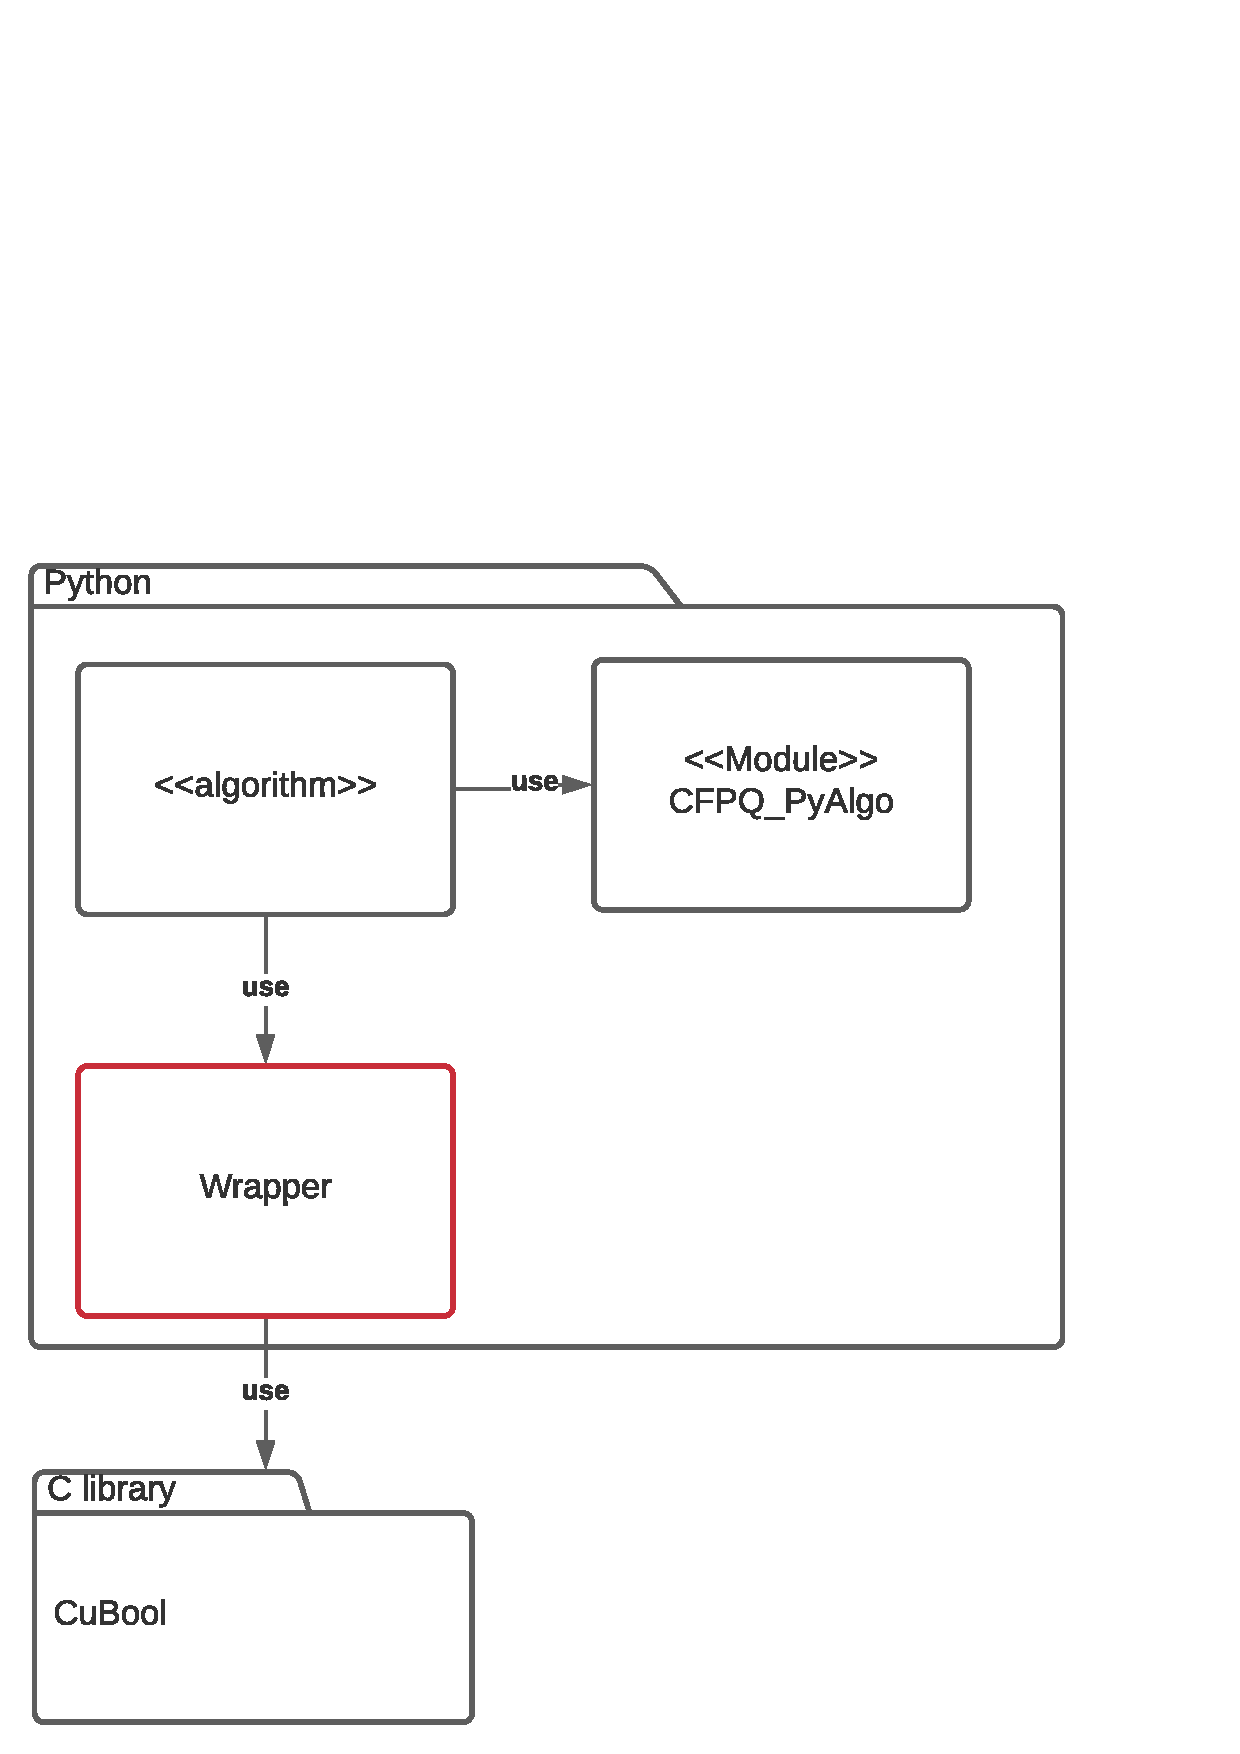
\includegraphics[width=15cm]{arch.png}
\caption{Архитектура решения}
\label{arch}
\end{center}
\end{figure}    

В следующих разделах будут детально описаны все шаги по использованию предложенного подхода.

\subsection{Подготовка входных данных}

В данном разделе описаны необходимые для использования ппедложенного подхода данные, а также детали их хранения и представления. В процессе апробации подхода были выведены некоторые общие требования, позволяющие наиболее эффективно и удобно проводить экспериментальные исследования. 

Все необходимые данные помещаются в некоторое облачное хранилище, откуда могут извлекаться по мере необходимости. Входные данные --- исследуемые цепочки --- последовательно записаны в файлы формата fasta (для, например, биологических данных) или любого аналогичного текстового формата, причем каждой цепочке соответствует уникальный числовой идентификатор. Вся остальная информация о цепочках (метаданные, принадлежность к тестовой или обучающей выборке, класс и др.) хранится в специальной ссылочной таблице с доступом по идентификатору. 

Кроме того, в процессе исследования могут понадобиться специфические скрипты для промежуточной обработки данных, например, выборка для обучения нейронной сети, изменение длин цепочек, фильтрация входных данных и др. Эти скрипты реализуются в модуле Data Processing и могут быть переиспользованы в похожих экспериментах.

\subsection{Генерация данных с помощью синтаксического анализатора}
В рамках предложенной архитектуры синтаксический анализатор --- консольная утилита, принимающая на вход грамматику, файл с цепочками и список желаемых выходных форматов. Опишем основные принципы его работы.

Синтаксический анализ -- процесс проверки выводимости некоторой подстроки в заданной грамматике. В контексте предложенного решения терминальными символами грамматики являются символы исследуемых последовательностей, правила грамматики описывают характерные особенности их вторичной структуры, а алгоритм синтаксического анализа используется для извлечения этих особенностей путем поиска всех выводимых подстрок для данной строки для всех нетерминалов. Наш подход не зависит от выбора конкретного алгоритма синтаксического анализа, однако в описанных ниже экспериментах мы предлагаем использовать разработанный в рамках проекта YaccConstructor~\cite{yacc} в лаборатории JetBrains~\cite{jetbrains} алгоритм, основанный на матричных операциях~\cite{Azimov:2018:CPQ:3210259.3210264}, который демонстрирует высокую производительность на практике в связи с использование параллельных вычислений.

Результатом работы матричного синтаксического анализатора для строки и фиксированного нетерминала является верхнетреугольная битовая матрица разбора. Мы предлагаем использовать такие матрицы как входные данные нейронной сети, поэтому необходимо привести их к удобному для обработки формату, учитывая специфику конкретной задачи. На данный момент в рамках расширения используемого алгоритма реализованы два формата преобразования матриц.
\begin{itemize}
    \item Вектора характеристик, сохраняемые в виде строк csv-файла. Генерация векторов осуществляется следующим образом: отбрасывается пустая часть матрицы ниже главной диагонали, оставшиеся строки последовательно преобразовываются в битовый вектор, а затем сжимаются в байтовый вектор.
    \item  Черно-белые изображения в формате bmp, получаемые путем замены нулевых битов матрицы на белые пиксели, а единичных --- на черные.
\end{itemize}
 %Пример преобразований представлен на рис.3. 
Кроме того, в исходный код инструмента можно легко добавить другие выходные форматы.

Классификация как векторов характеристик, так и изображений относится к классическим сценариям использования нейронных сетей, однако стоит отметить, что ввиду специфики конкретной задачи и особенностей входных цепочек, выбор формата данных может повлиять на эффективность и скорость обучения. Например, в процессе экспериментальных исследований было обнаружено, что несмотря на то, что векторные данные занимают меньше памяти и ускоряют процесс обучения, их использование предполагает выравнивание всех цепочек до одинаковой длины, что может оказаться не самым эффективным решением для задач, где входные последовательности имеют принципиально разные длины, так как большая часть вектора для коротких цепочек в данном случае будет заполнена незначащими нулями. Изображения же можно сгенерировать для цепочек разных длин и затем привести к одному разрешению, что позволяет аккуратно сохранить особенности вторичной структуры даже для коротких цепочек, однако это приводит к ухудшению скорости обучения и вызывает необходимость хранения больших объемов данных. 

\subsection{Обучение нейронных сетей}
Искуственные нейронные сети -- широко применямый метод решения задач классификации в областях, где входные данные обладают сложно формализуемыми закономерностями и могут содержать шумы и неточности. Мы предлагаем использовать нейронные сети для обработки сгенерированных синтаксическим анализатором данных, предполагая, что в них закодированы существенные для классификации особенности синтаксической структуры.

Архитектура нейронной сети уникальна для каждой конкретной задачи и предметной области, однако экспериментальные исследования выявили некоторые общие закономерности и интуиции. Для векторизованных данных высокую эффективность показало чередование полносвязных (dense) слоев ввиду утери информации о взаимном расположении элементов изначальной битовой матрицы и дропаут (dropout) слоев с нормализацией для разжатия данных. Для изображений мы предлагаем использовать небольшое количество сверточных слоев (так как они применяются в основном для извлечения каких-либо особенностей из входных данных, а в нашем случае это уже сделано на этапе синтаксического анализа), затем линеаризацию, а далее перейти к чередующимся dense и dropout слоям, аналогично архитектуре для веторизованных данных.

Выше был описан стандартный в рамках нашего подхода способ использования нейронных сетей, однако возможны различные его модификации, основанные на констуировании более сложных моделей с загрузкой весов уже обученных, что позволяет упростить задачу или повысить точность результата. Например, расширение нижней части нейронной сети слоями с большим количеством нейронов позволяет провести классификацию на большее количество классов, а расширение верхней части предоставляет возможность подачи на вход данных в другом формате, например, изначальной символьной последовательности вместо результата парсинга.

Остановимся подробнее на последней модификации. Большинство алгоритмов синтаксического анализа работают за полином от длины входа, поэтому генерация большого количества данных на длинных цепочках потребует существенных временных затрат. Поэтому мы предлагаем следующую идею.
\begin{itemize}
    \item Сгенерировать некоторый набор данных с помощью синтаксического анализатора и обучить на них нейронную сеть (NN1).
    \item Создать новую нейронную сеть (NN2), которая расширяет вход NN1 несколькими слоями, верхний из которых принимает символьные цепочки.
    \item Подгрузить веса NN1 на нижнюю часть NN2 и дообучить NN2.
\end{itemize}

Эта идея может быть применена как к векторизованным данным, так и к изображениям. В случае изображений необходимо использовать веса NN1, начиная с линеаризованного слоя. Таким образом можно, во-первых, уменьшить размер выборки для генерации парсером, а во-вторых, улучшить точность уже обученных нейронных сетей без временных затрат на дополнительную генерацию данных. Высокая точность и скорость обучения такой нейронной сети была подтверждена экспериментальным путем. 

\section*{Заключение}
В ходе данной работы были получены следующие результаты.
\begin{itemize}
    \item Раработана архитектура решения для использования предложенного подхода.
    \item Проведены экспериментальные исследования предложенного подхода на задачах распознавания 16s рРНК и классификации тРНК.
    \item Задокументировано описание схемы работы подхода и результаты проведенных экспериментов.
    \item Опубликована статья "The Composition of Dense Neural Networks and Formal Grammars for Secondary Structure Analysis" на конференции BIOINFORMATICS 2019
    \item Представлен постер "16s rRNA Detection by Using Neural Networks" на конференции Biata 2018
\end{itemize}

Существует несколько направлений дальнейшего развития получен-
ных результатов.
\begin{itemize}
    \item Эксперименты в области кибербезопасности --- поиск анмалий в последовательностях системных вызовов.
    \item Предсказание функций белков.
    \item Распознавание химер.
    \item Моделирование вторичной структуры геномных пследовательностей
    \item Рибозимы???
\end{itemize}


% У заключения нет номера главы
%\section*{Coclusion}

\setmonofont[Mapping=tex-text]{CMU Typewriter Text}
\bibliographystyle{ugost2008ls}
\renewcommand\refname{Список литературы}
\bibliography{diploma.bib}
\end{document}
